\documentclass{beamer}

\usepackage{multirow}
\usepackage{booktabs}
\usepackage[]{algorithm}
\usepackage{algpseudocode}
\usepackage{dirtytalk}
\usepackage{csquotes}
\usepackage{lineno,hyperref}
\usepackage{amsmath} 
\usepackage{amssymb}% http://ctan.org/pkg/amssymb
\usepackage{pifont}
\usepackage{graphicx}
\usepackage{subcaption}
\usepackage{multirow}
\usepackage{booktabs}
\usepackage{tabularx}
\usepackage{rotating}
\usepackage{adjustbox}
\usepackage{lscape}
\usepackage{longtable}
\usepackage{algpseudocode}
\usepackage[]{algorithm}
\usepackage{textcomp}

\usepackage[sharp]{easylist}
\usepackage{adjustbox}

\usetheme{Madrid}
\definecolor{tecBlue}{rgb}{0, .3333, .65098}
\usecolortheme[named=tecBlue]{structure}

\title[Master's Degree Thesis]{Comparison between Single Objective and Multi Objective Algorithms for the creation of stable student groups.}

\subtitle{Master's Degree Thesis}

\author{Miguel Angel Bravo Vidales}

\institute[] 
{School of Engineering and Sciences \\
  Computer Science}

\date{September, 2019}
\pgfdeclareimage[height=.5cm]{university-logo}{images/logo_tec}
\logo{\pgfuseimage{university-logo}}

% Delete this if you do not want the table of contents to pop up at
% the beginning of each subsection:

\AtBeginSection[]
{
  \begin{frame}<beamer>{Outline}
    \tableofcontents[currentsection]
  \end{frame}
}

% Maybe... hwere to put not in each subsection but at least in each section


\begin{document}

\begin{frame}
  \titlepage
\end{frame}

\begin{frame}{Outline}
%   \tableofcontents[pausesections]
  \tableofcontents
\end{frame}

\section{Introduction}

    \subsection{Motivation}
    \begin{frame}{Motivation}
        \begin{itemize}
            \item  People still learning a foreign language such as English have a need to practice it. 
            \item One of the best way to do this is by having a casual conversation in a small group.
            \item For this a platform was proposed that can enable them to have a casual conversation with unknown people.
            \item One of the problems that arise from this is that, the people within these groups have a preference to which persons they may want to establish a conversation with.
        \end{itemize}
    \end{frame}
    
    \begin{frame}{Motivation} % Check this part (i think its unnecessary)
        \begin{itemize}
            \item This personal preference includes:
            \begin{itemize}
                \item Students may want to have a conversation about a certain topic
%which sometimes may be unknown or irrelevant to the rest of the group.
                \item Students may have a different level of experience in the English speaking.
            \end{itemize}
        \item In addition there are two additional constraints for the benefit of the system.
            \begin{itemize}
                \item The groups should not be too big nor small
%to ensure that the conversation can be maintained.
                \item It's necessary that all the people within the group participate in the conversation.
        \end{itemize}
    \end{itemize}
    \end{frame}

    \subsection{Hypothesis}
    \begin{frame}{Hypothesis}
        Multi-Objective algorithms can outperform Single Objective algorithms in finding stable studying groups based on their interests and level of experience and considering the group size and the participation as constraints.\\
    \end{frame}
    \begin{frame}{Hypothesis}
    The research aims to answer the following questions
        \begin{itemize}
            \item How can the structure of this problem be defined in terms of optimisation? 
            \item How much can improve an optimised solution from a initial random one? % <- ? 
            \item In which scenarios can a Single Objective algorithm outperform multi objective algorithms?
            \item Among Single and Multi Objective algorithms which one results to be the best suited for the problem overall?
        \end{itemize}
    \end{frame}
    
    \subsection{Objective}
    \begin{frame}{Objective}
        Define the problem's structure as well as its objective functions to optimise the stability (preference) of the users and the system. And Determine which Strategy whether Single-objective or Multi-Objective is better suited for this optimisation.
    \end{frame}
    
\section{Methodology}

    \subsection{Problem Definition}
    \begin{frame}{Problem Definition}
        Given a Data set of users of size N, find the optimal way to arrange them in groups according to their preferences.\\
    
        A solution of this problem must have every user of the data set in a group with their preferences optimised.\\
    \end{frame}

        %(because the users are unknown to each other, this preferences are assumed)  
        
        % In another Slide...
    \begin{frame}{Problem Definition}
        In this particular research, the preference is defined as:
        \begin{itemize}
            \item Having similar interests.
            \item Having a similar level of experience speaking the English language.
        \end{itemize}

        
        In addition the problem has the following constraints for the benefit of the system:
        \begin{itemize}
            \item The groups must near the "ideal size" which in this problem is between 4 to 5 members.
            \item The groups must have an homogeneous participation of each of its members.
        \end{itemize}
    \end{frame}
    
    \begin{frame}{Similar Problems}
        % Image?
        % https://miro.medium.com/max/1086/1*ME9Qli0uDQiDQD0hsaIiug.png
        % http://mathworld.wolfram.com/images/eps-gif/StableMarriage_1000.gif
        % Given $n$ men and $n$ women, where each person has ranked all members of the opposite sex in order of preference, marry the men and women together such that there are no two people of opposite sex who would both rather have each other than their current partners. When there are no such pairs of people, the set of marriages is deemed stable. [Ref(Gale, D. and Shapley)]\\ 
        
        %Other similar problems:
        
        \begin{itemize}
            \item Stable Marriage Problem \cite{10.2307/2312726,McVitie:1971:SMP:362619.362631}
            \item Stable Roommates problems \cite{ROTH2005151,Irving:2007:CRP:1240328.1240414,kujansuu1999stable}
            \item Hospitals/residents problem \cite{gale1985some,roth1984evolution,gusfield1989stable}
            \item \textbf{Hospitals/residents problem with couples} \cite{McDermid2010,10.1007/978-3-319-07959-2_2}
            \item Matching with contracts \cite{matching_with_contracts}
        \end{itemize}
        
    \end{frame}

    \subsection{Preference Criteria | Objective Functions}
    \begin{frame}{Experience Level | CEFR}
        \begin{figure}
            \centering
            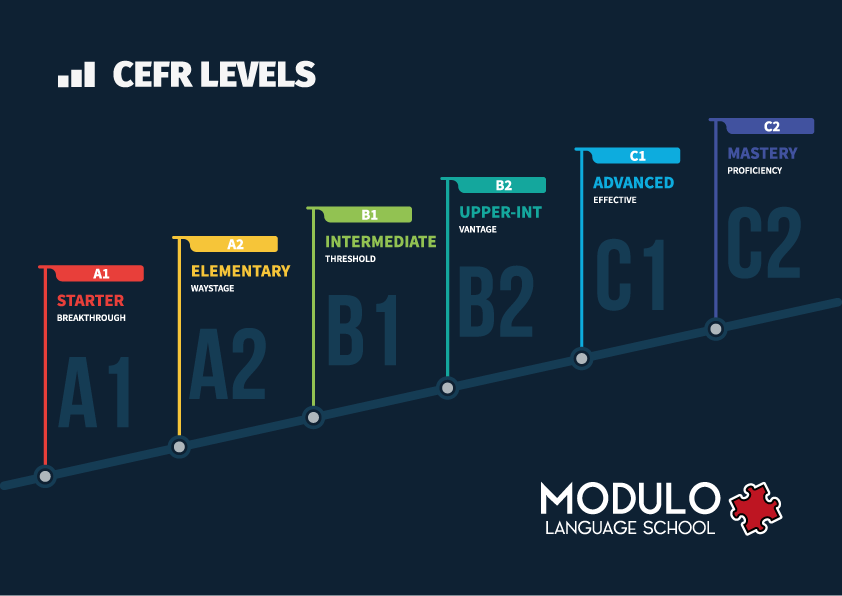
\includegraphics[width=0.8\textwidth]{images/cefr-levels.png}
            \footnote{https://www.modulolearning.com/modulo-cefr-levels.html} 
        \end{figure}\\ 
%        Common European Framework of Reference for Languages  is an international standard for describing language ability [ref]
    \end{frame}
    
    \begin{frame}{Interest Similarity | Facebook Ad Platform}
        \begin{figure}
            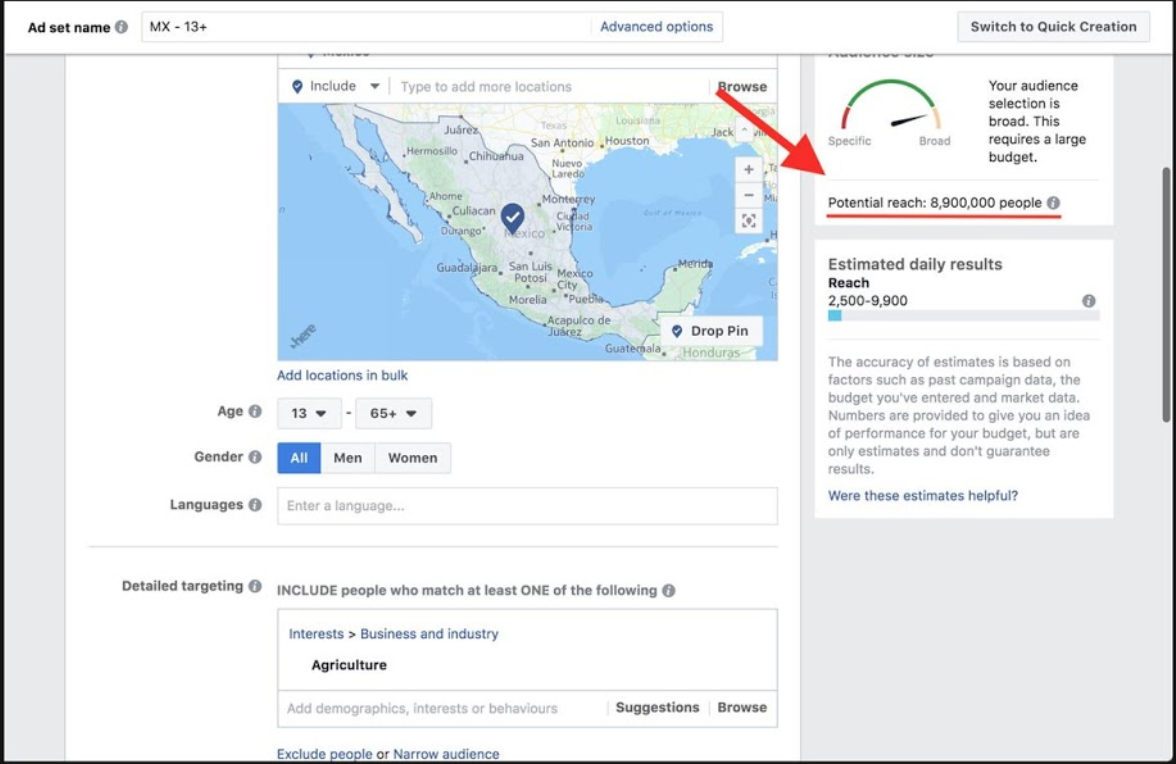
\includegraphics[width=\textwidth]{images/facebook.png}
        \end{figure}
    \end{frame}
    
    \begin{frame}{Interest Similarity | Facebook Ad Platform}
        \begin{figure}
            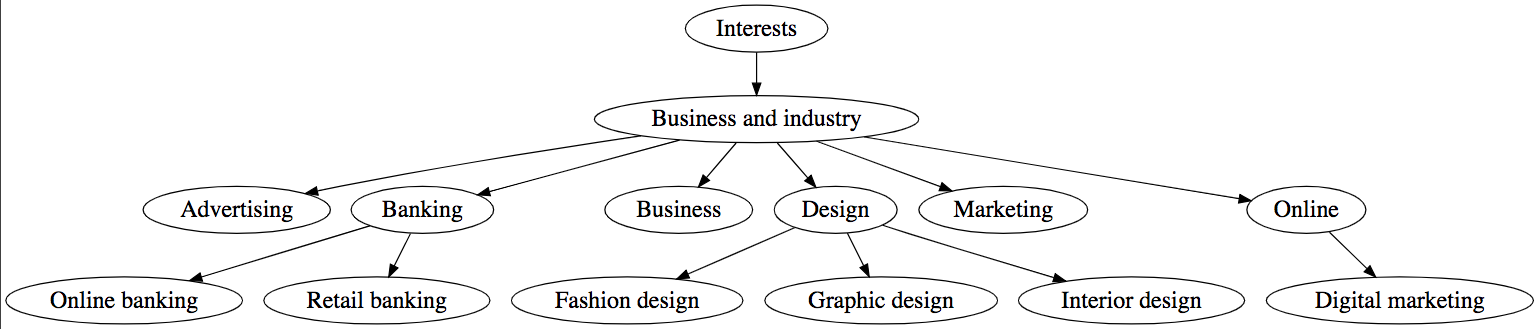
\includegraphics[width=\textwidth]{images/ontology.png}
        \end{figure}
    
        Facebook possess an ontology of interests which puts similar interests in the same branch, in addition this each interest in this category has a proportion according to the population that has said interest.
    \end{frame}
    
    \begin{frame}{Participation Percentage | AMI Meeting Corpus}
    
            \begin{columns}
                \begin{column}{0.50\textwidth}
                    \begin{figure}
                        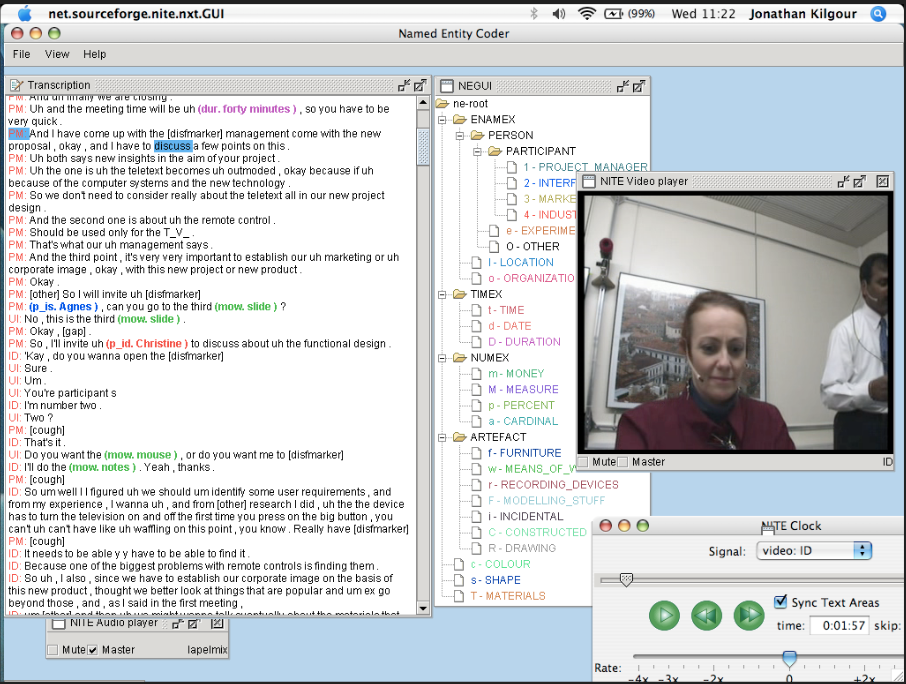
\includegraphics[width=\textwidth]{images/ami.png}
                        % May be changed for an actual table
                    \end{figure}
                \end{column}
                \begin{column}{0.50\textwidth}
                    \begin{figure}
                        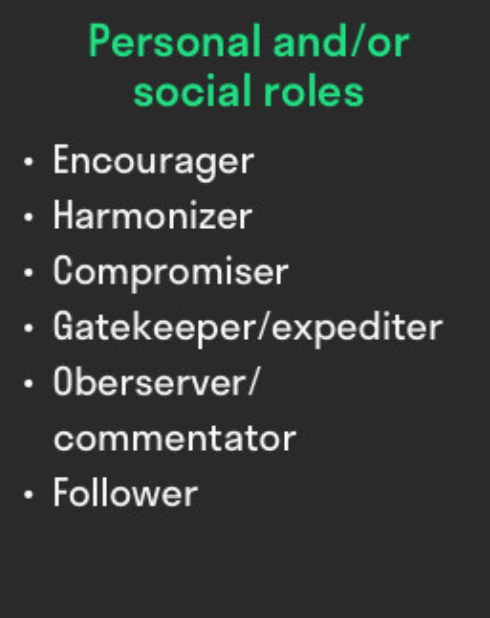
\includegraphics[width=0.7\textwidth]{images/roles.png}
                    \end{figure}
                \end{column}
            \end{columns}\\
    
        The corpus \cite{carletta2005ami} is a dataset of several conversations labeled according to Benne and Sheats Functional Roles definition \cite{benne1948functional}
    \end{frame}
    
    \begin{frame}{Synthetic Data set}
        \begin{figure}
            \centering
            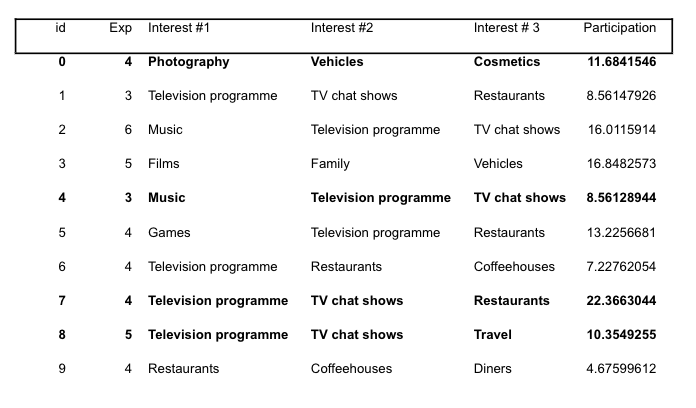
\includegraphics[width=0.8\textwidth]{images/dataset.png}
        \end{figure}
    \end{frame}
    \begin{frame}{Synthetic Data set}
        \begin{itemize}
            \item The preference Criteria also served as the basis for the creation of the different data sets
            \item Each data set has a size of n {20, 200, 2,000, 10,001}, each generated randomly according to Mean and Standard Deviation found for each attribute
        \end{itemize}
    \end{frame}
    
    \subsection{Evolutive Algorithms and Single Objective Metaheuristics}
    
    \subsection{Comparison Between Single and Multi Objective Optimisation Algorithms}
    \begin{frame}{Comparison Between Single and Multi Objective Optimisation Algorithms}
    
            \begin{columns}
                \begin{column}{0.50\textwidth}
                    \begin{figure}
                        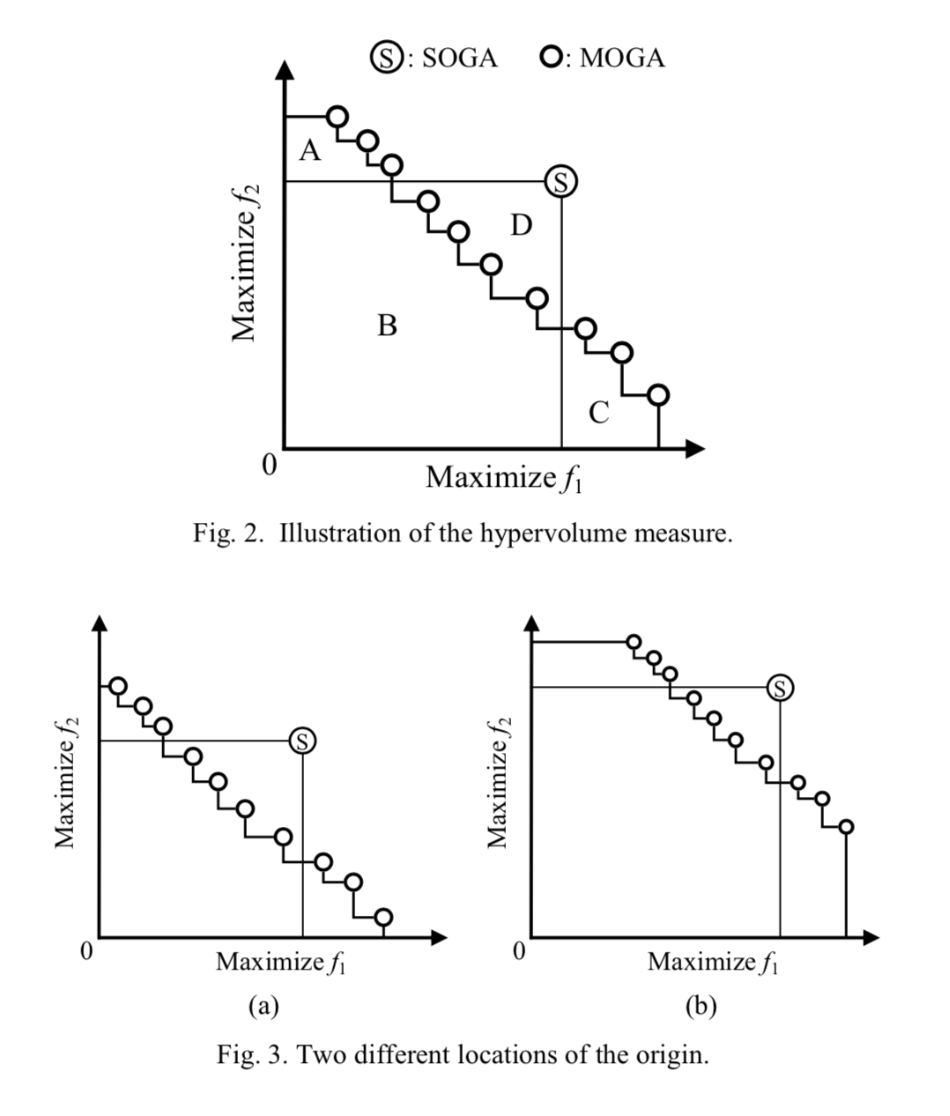
\includegraphics[width=0.8\textwidth]{images/hv.png}
                    \end{figure}
                \end{column}
                \begin{column}{0.50\textwidth}
                    \begin{figure}
                        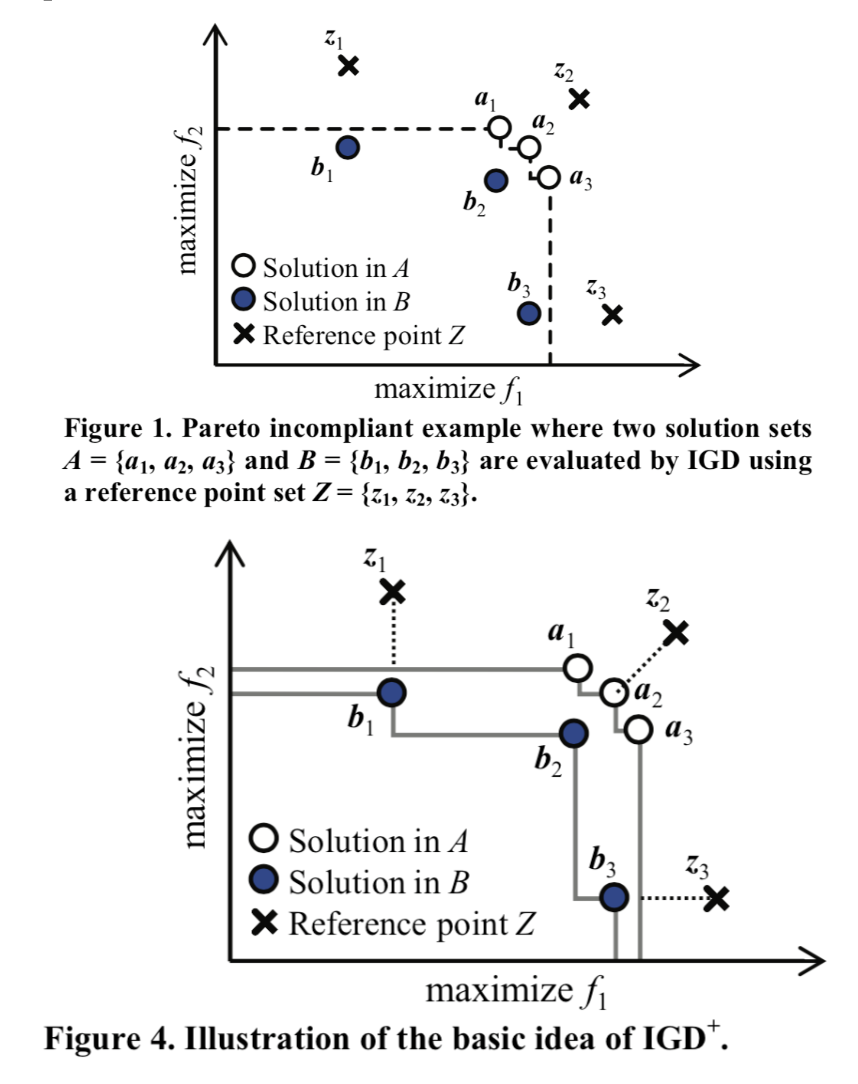
\includegraphics[width=0.7\textwidth]{images/igd+.png}
                    \end{figure}
                \end{column}
                \footnote{H. Ishibuchi, Y. Nojima, and Tsutomu Doi, “Comparison betweensingle-objective and multi-objective genetic algorithms:  Performancecomparison and performance measures,” in2006 IEEE InternationalConference on Evolutionary Computation, pp. 1143–1150, July 2006.}
            \end{columns}\\
    
        %\begin{itemize}
        %    \item Several of the works made by H. Ishibuchi et al [ref], includes a comparison between single %objective and multi-objective algorithms
        %    \item One of the challenges about comparing the performance is choosing an adequate performance measure, %while HV is usually the most common for MOGA's, Ishibuchi suggests using IGD+ for a better comparison to SOGA's
        %\end{itemize}
    \end{frame}

    \section{Experiments and Results}
    \subsection{Experimental Parameters}
    \begin{frame}{Is it even optimising?}
        \begin{figure}
            \centering
            % Rebuild Graph and include parameters...
            \caption{Single Objective Local Search Algorithm}
            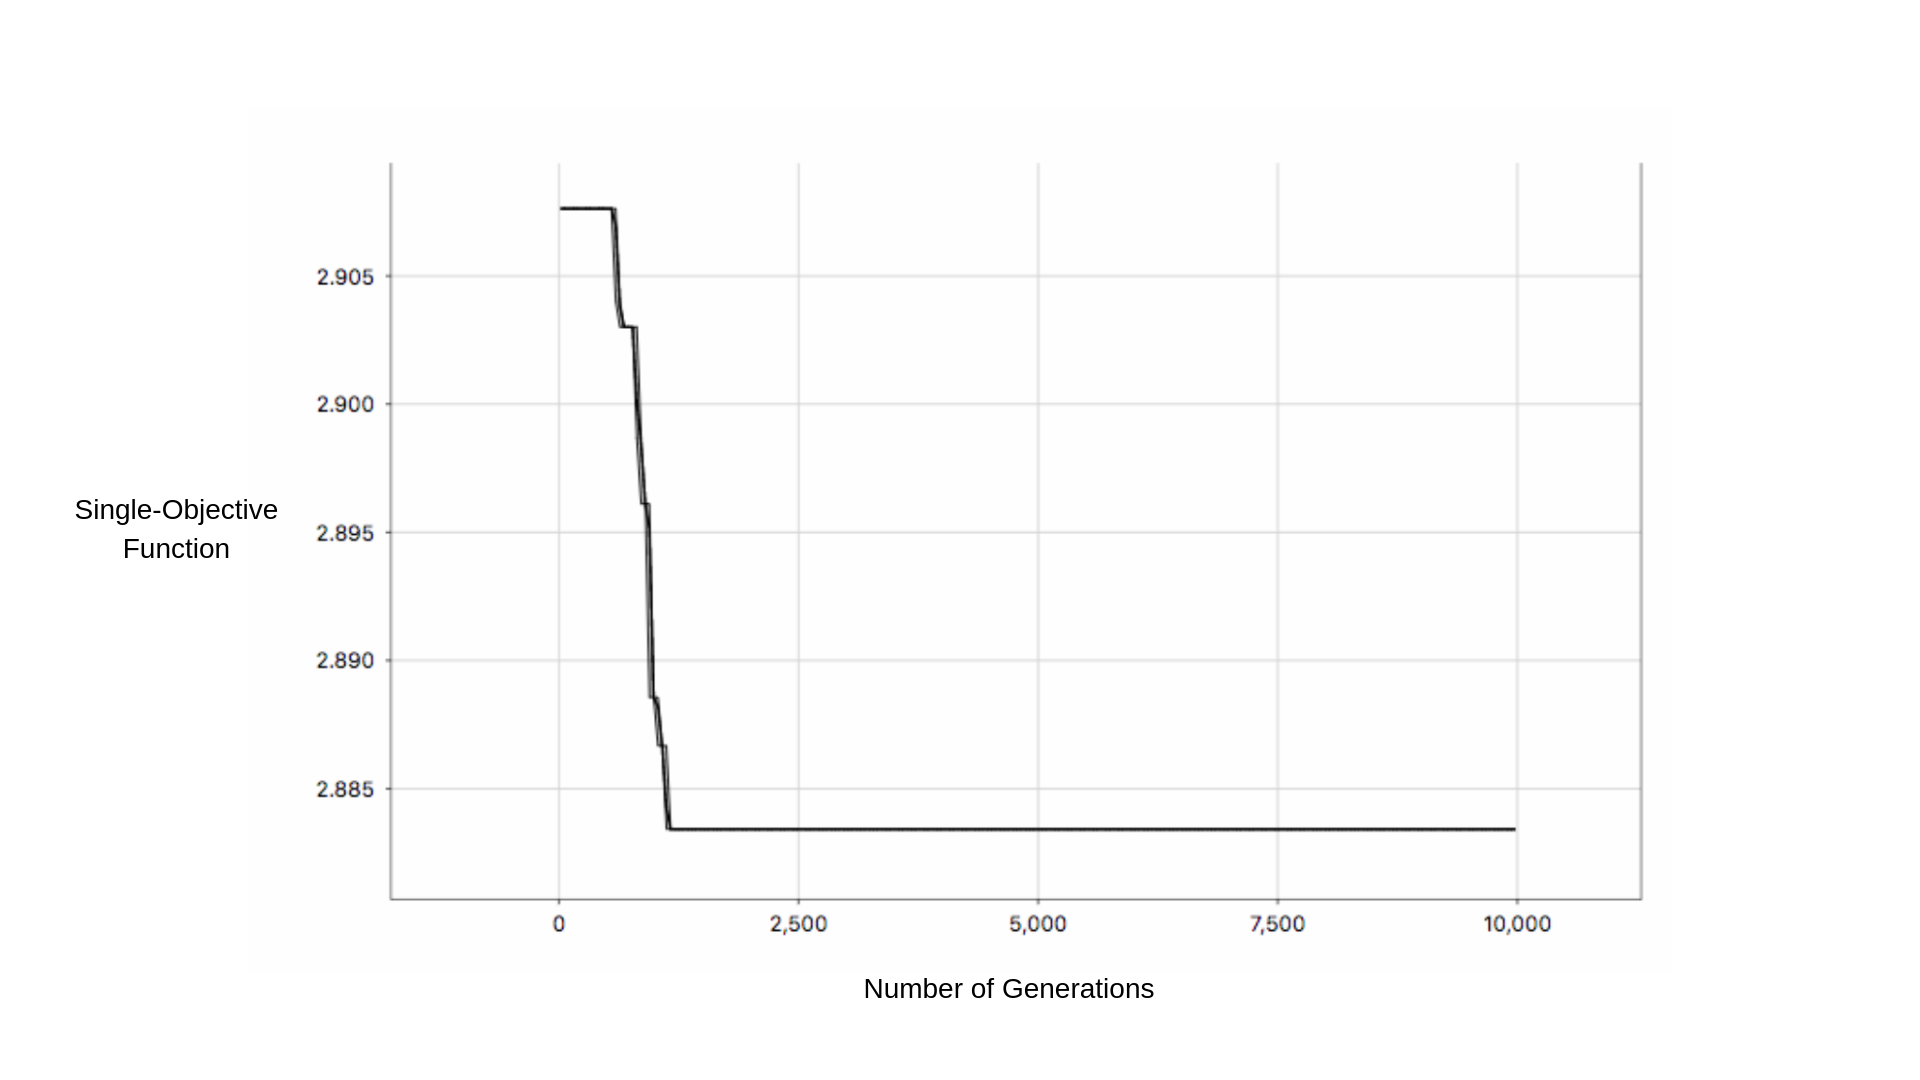
\includegraphics[width=\textwidth]{images/localsearch.png}
        \end{figure}
    \end{frame}
    
    \subsection{Comparison between SOOA's and MOOA's}
       \begin{frame}{Experiment Parameters}
        All algorithms were executed with similar parameters
        \begin{itemize}
            \item A population of $n = 100$ % (in the case of population algorithms)
            \item A number of evaluations of $100*n$ % (for optimisation meta heuristics this was $100*n$ steps)
        \end{itemize}\\
        \\
        \\
        \begin{columns}
                \begin{column}{0.50\textwidth}
                    \\
                    The Single-Objective algorithms:
                    \begin{itemize}
                        \item Local Search % (Steepest Descent/Hill Climbing)
                        \item Random Search
                        \item Random Descent % (Stochastic Hill Climbing)
                        \item Genetic Generational Algorithm
                        \item Genetic Steady Algorithm 
                        \item Elitist Algorithm $(\mu+\lambda)$ 
                        \item Non-Elitist Algorithm $(\mu,\lambda)$
                    \end{itemize}
                \end{column}
                \begin{column}{0.50\textwidth}
                    The Multi-Objective algorithms:
                    \begin{itemize}
                        \item ESPEA 
                        \item MOMBI2
                        \item NSGAII
                        \item RS    
                        \item SPEA2 
                    \end{itemize}
                \end{column}
            \end{columns}\\
    \end{frame}
    
    
    % Single-Objective
    \begin{frame}{Results / Single-Objective / $n=20$}
            \begin{columns}
                \begin{column}{0.70\textwidth}
                    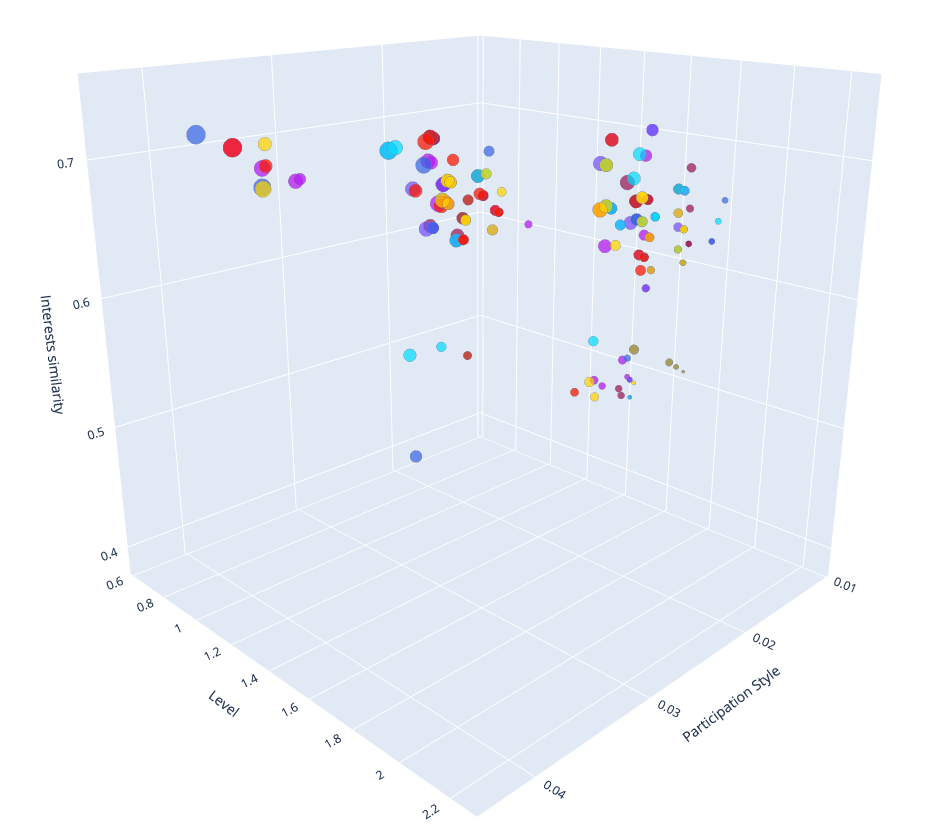
\includegraphics[width=\textwidth]{images/20_single.png}
                \end{column}
                \begin{column}{0.30\textwidth}
                    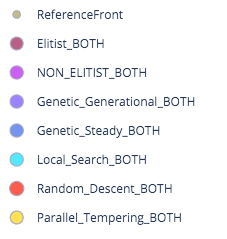
\includegraphics[width=\textwidth]{images/legend_single.png}
                \end{column}
            \end{columns}\\
    \end{frame}
    
    \begin{frame}{Results / Single-Objective / $n=200$}
            \begin{columns}
                \begin{column}{0.70\textwidth}
                    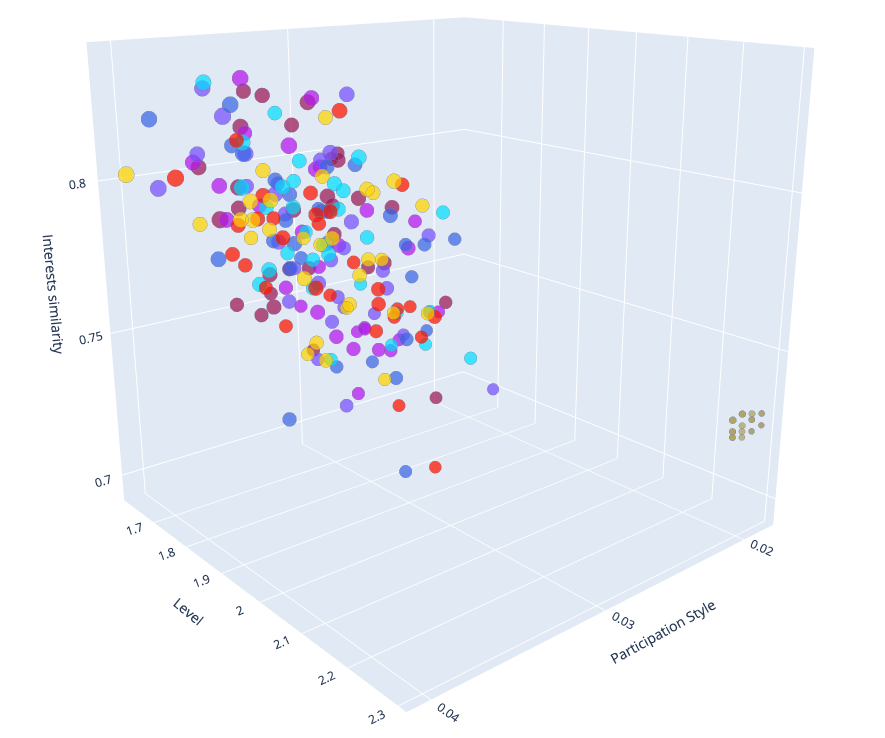
\includegraphics[width=\textwidth]{images/200_single.png}
                \end{column}
                \begin{column}{0.30\textwidth}
                    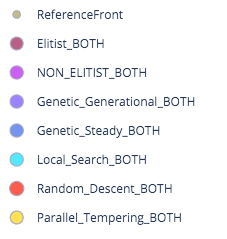
\includegraphics[width=\textwidth]{images/legend_single.png}
                \end{column}
            \end{columns}\\
    \end{frame}
    
    \begin{frame}{Results / Friedman Test IGD+}
        \begin{table}[!htp]
            \centering
            \caption{Average ranking of the algorithms}
            \begin{tabular}{c|c}
            Algorithm&Ranking\\
            \hline
            Random Descent&5.75\\
            \textbf{Parallel Tempering}&\textbf{3.0}\\
            Random Search&3.75\\
            Local Search&4.5\\
            Genetic Steady&5.0\\
            Genetic Generational&5.25\\
            Elitist&5.0\\
            NON ELITIST&3.75\\
            \end{tabular}
        \end{table}
        Friedman statistic considering reduction performance (distributed according to chi-square with 7 degrees of freedom: \textbf{4.0}).
    \end{frame}
    
    % Multi-Objective
    \begin{frame}{Results / Multi-Objective / $n=20$}
            \begin{columns}
                \begin{column}{0.70\textwidth}
                    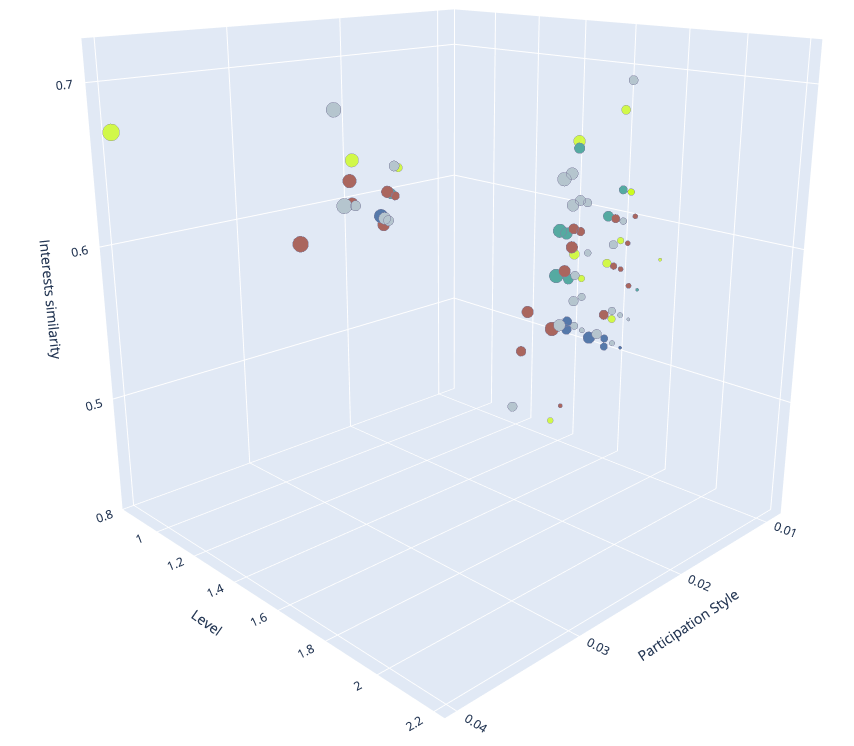
\includegraphics[width=\textwidth]{images/20_multi.png}
                \end{column}
                \begin{column}{0.30\textwidth}
                    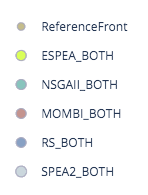
\includegraphics[width=\textwidth]{images/legend_multi.png}
                \end{column}
            \end{columns}\\
    \end{frame}
    
    \begin{frame}{Results / Multi-Objective / $n=200$}
            \begin{columns}
                \begin{column}{0.70\textwidth}
                    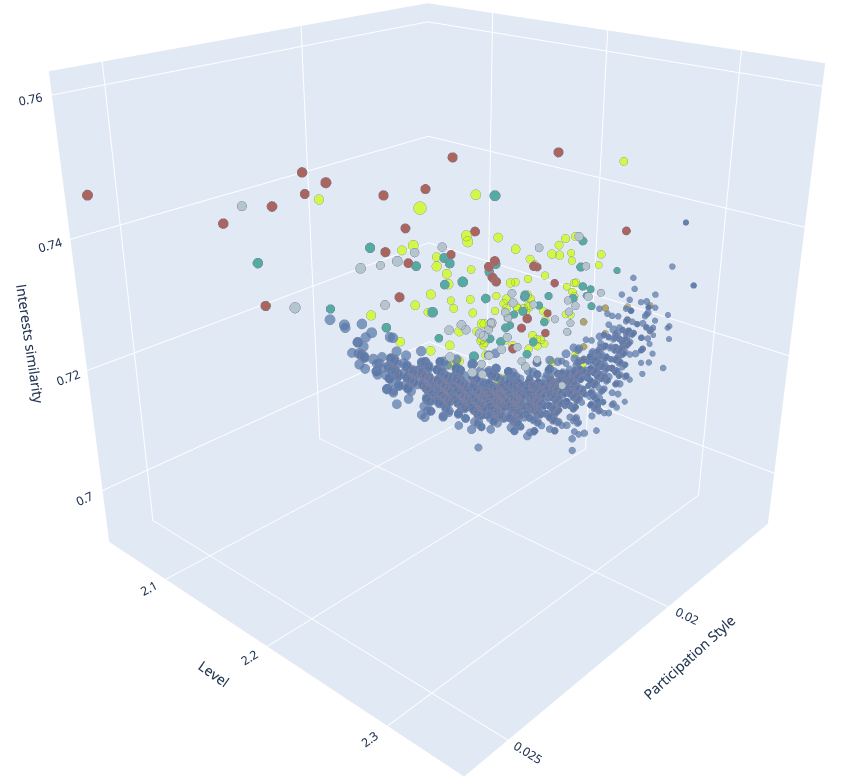
\includegraphics[width=\textwidth]{images/200_multi.png}
                \end{column}
                \begin{column}{0.30\textwidth}
                    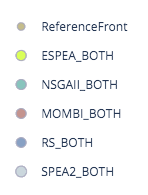
\includegraphics[width=\textwidth]{images/legend_multi.png}
                \end{column}
            \end{columns}\\
    \end{frame}
    
    \begin{frame}{Results / Friedman Test IGD+}
        \begin{table}[!htp]
            \centering
            \caption{Average ranking of the algorithms}
            \begin{tabular}{c|c}
            Algorithm&Ranking\\
            \hline
            ESPEA&3.0\\
            MOMBI&4.25\\
            NSGAII&3.0\\
            \textbf{RS}&\textbf{1.0}\\
            SPEA2&3.75\\
            \end{tabular}
        \end{table}

    Friedman statistic considering reduction performance (distributed according to chi-square with 4 degrees of freedom: \textbf{9.8}).
    \end{frame}
    
    
    % Single vs Multi-Objective
    \begin{frame}{Results / Single vs Multi / $n=20$}
            \begin{columns}
                \begin{column}{0.70\textwidth}
                    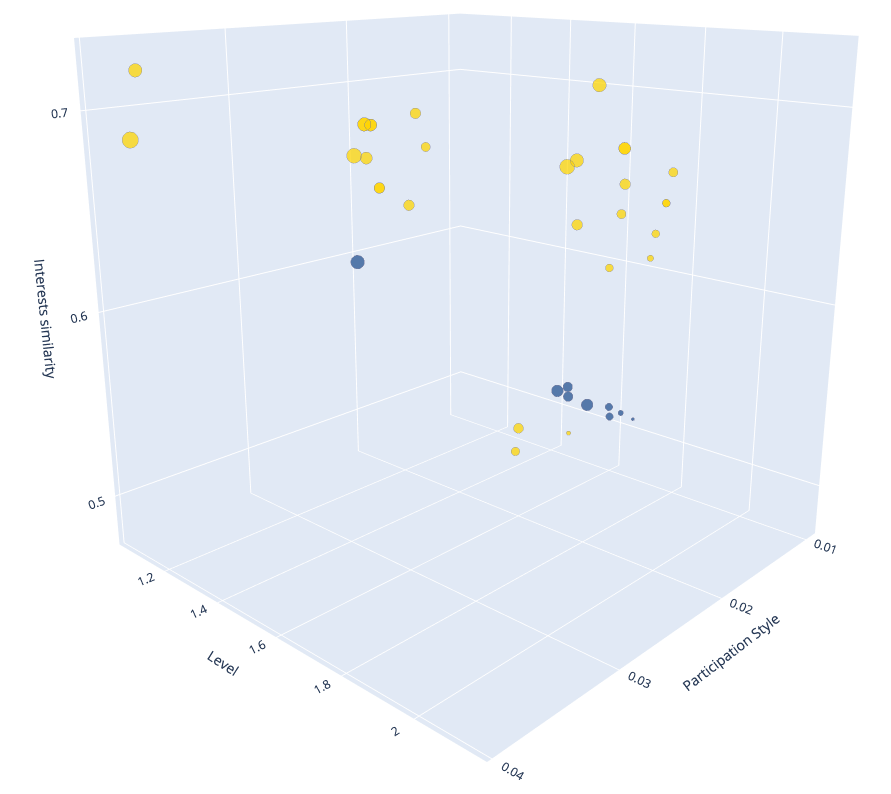
\includegraphics[width=\textwidth]{images/20_both.png}
                \end{column}
                \begin{column}{0.30\textwidth}
                    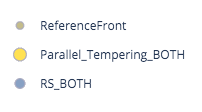
\includegraphics[width=\textwidth]{images/legend_both.png}
                \end{column}
            \end{columns}\\
    \end{frame}
    
    \begin{frame}{Results / Single vs Multi / $n=200$}
            \begin{columns}
                \begin{column}{0.70\textwidth}
                    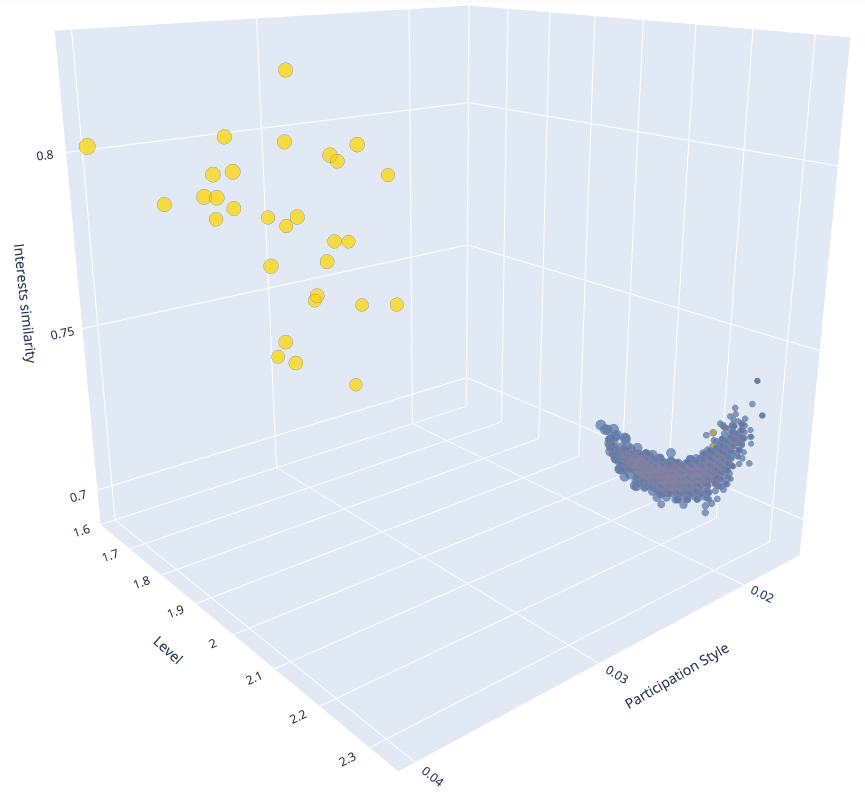
\includegraphics[width=\textwidth]{images/200_both.png}
                \end{column}
                \begin{column}{0.30\textwidth}
                    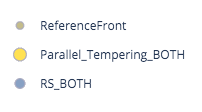
\includegraphics[width=\textwidth]{images/legend_both.png}
                \end{column}
            \end{columns}\\
    \end{frame}
    
    \begin{frame}{Results / Friedman Test IGD+}
        \begin{table}[!htp]
            \centering
            \caption{Average ranking of the algorithms}
            \begin{tabular}{c|c}
            Algorithm&Ranking\\
            \hline
            \textbf{RS}&\textbf{1.0}\\
            Parallel Tempering&2.0\\
            \end{tabular}
        \end{table}
    
    
        Friedman statistic considering reduction performance (distributed according to chi-square with 1 degrees of freedom: \textbf{4.0}).
    \end{frame}
    
    % Single vs Multi-Objective
    \begin{frame}{Results / Single vs Multi (Corrected) / $n=20$}
            \begin{columns}
                \begin{column}{0.70\textwidth}
                    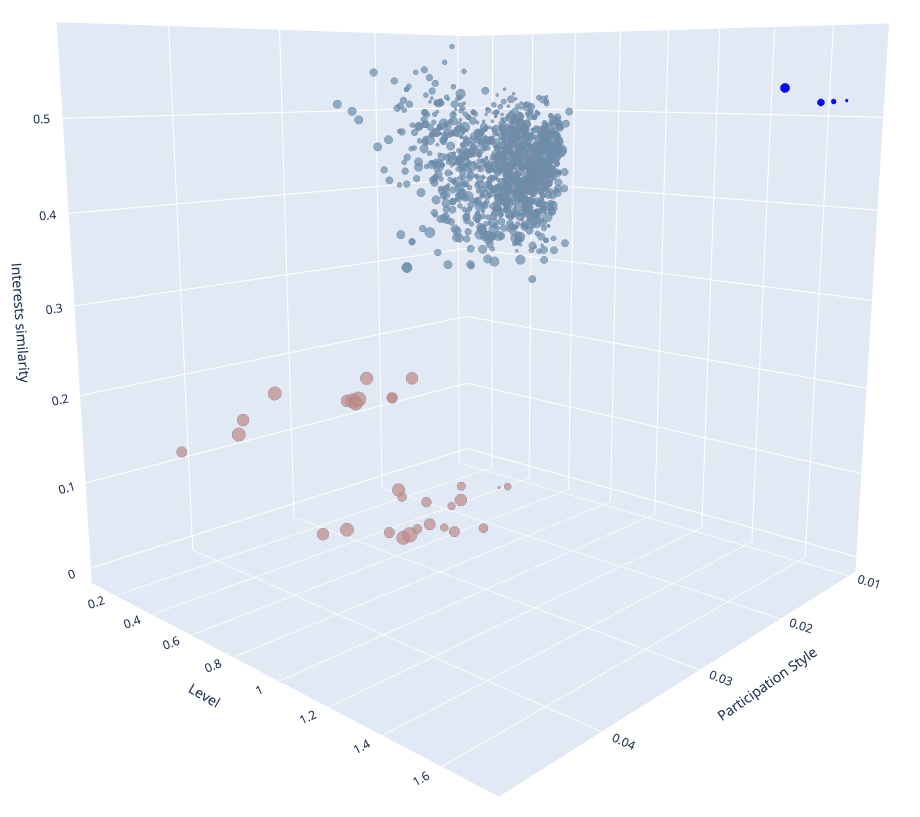
\includegraphics[width=\textwidth]{images/20_both_rev.png}
                \end{column}
                \begin{column}{0.30\textwidth}
                    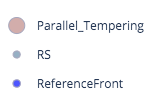
\includegraphics[width=\textwidth]{images/legend_both_rev.png}
                \end{column}
            \end{columns}\\
    \end{frame}
    
    \begin{frame}{Results / Single vs Multi (Corrected) / $n=200$}
            \begin{columns}
                \begin{column}{0.70\textwidth}
                    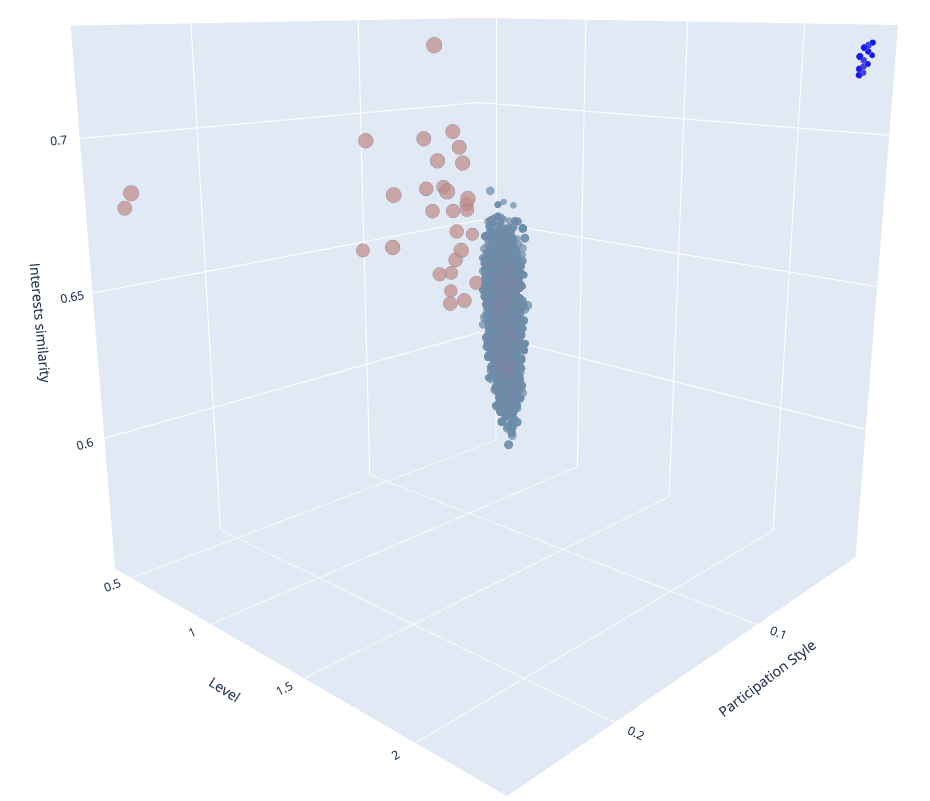
\includegraphics[width=\textwidth]{images/200_both_rev.png}
                \end{column}
                \begin{column}{0.30\textwidth}
                    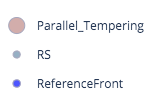
\includegraphics[width=\textwidth]{images/legend_both_rev.png}
                \end{column}
            \end{columns}\\
    \end{frame}
    
    \begin{frame}{Results / IGD+ for the 20 Problem}
        \begin{table}
        \caption{IGD+. Mean and Standard Deviation}
        \label{table: IGD+}
        \centering
        \begin{scriptsize}
        \begin{tabular}{lllllllllllll}
        \hline & RS & Parallel Tempering \\
        \hline 
        Grouping\_Problem\_20 & \textbf{$  5.98e-02_{ 3.0e-02}$} & $  5.56e+00_{ 2.6e+00}$  \\
        \hline
        \end{tabular}
        \end{scriptsize}
        \end{table}
        
        \begin{table}
        \caption{IGD+. Median and Interquartile Range}
        \label{table: IGD+}
        \centering
        \begin{scriptsize}
        \begin{tabular}{lll}
        \hline & RS & Parallel Tempering \\
        \hline 
        Grouping\_Problem\_20 & \textbf{$ 5.89e-02_{ 2.9e-02}$} & $5.61e+00_{ 3.1e+00}$ \\
        \hline
        \end{tabular}
        \end{scriptsize}
        \end{table}
    \end{frame}
    
    \section{Conclusions}
    \begin{frame}{Conclusions}
        \begin{itemize}
            \item  SOOA's can outperform MOOA's given a small enough problem, however when the size of the problem increases MOOA's outperform SOOA's and SOOA's surpassing MOOA's is not consistent
            \item Four objectives doesn't seem to affect the performance of MOOA's
            \item RS was highlighted as the most competitive, however it gets away from the reference front with a high size of the problem
            \item This could be explained because of the homogeneous distribution of the database, as most of its  values have little variance.
            \item It could also be explained by the discrete nature of the problem.
        \end{itemize}
    \end{frame}
    
    \section{Future work}
    \begin{frame}{Future work}
        \begin{itemize}
            \item Relaxed Constraints
            \item Parameter tuning
            \item Prove with a real data set
            \item Compare to other Clustering strategies eg. "Multi-Objective Clustering and Cluster Validation" by Julia Handl % Mention...
            \item Other Applications
        \end{itemize}

    \end{frame}
        
    \section*{References}
    \begin{frame}[allowframebreaks]
      \frametitle{References}
      \bibliographystyle{ieeetr}
      \bibliography{ref}
    \end{frame}    
    
\end{document}